\section{Memory consistency}
    \begin{tcolorbox}[vert]
        Cache coherence simulate a unique shared memory, so we don't have to think about the location of different data. \important{Memory consistency} determine in which order instructions are simulated, because the processor can re-order instructions, we have to take care about memory consistency. It tells which re-ordering operations are acceptable or not.

    The memory consistency affects performance!!
    \end{tcolorbox}
    
    To express this we can just look at this example
    \hypertarget{consistency}{}
    \begin{tcolorbox}[rouge]
        If we want to execute this two pieces of code, one in a processor, the other in another.

        \vspace{1em}
    \begin{minipage}{0.48\textwidth}
        \begin{codeCenter}
        \begin{Ccode}
// A = r0 = 0
(S0) A = 1;
(L0) r0 = B;
print(r0);           
        \end{Ccode}
        \end{codeCenter}
    \end{minipage}
    \begin{minipage}{0.48\textwidth}
        \begin{codeCenter}
        \begin{Ccode}
// B = r1 = 0
(S1) B = 1;
(L1) r1 = A;
print(r1);
        \end{Ccode}
        \end{codeCenter}
    \end{minipage}
    \end{tcolorbox}

    We can obtain $\left(0,0\right)$ as result, but we don't expect that. Why we can obtain this? Because processors can execute this code like this
    \begin{image}{First, A and B are in shared state in both processors, then processors execute the stores simultaneously. While value are in the storing process, non-blocking caches proceed and the read hits. It returns $\left(0,0\right)$.}
        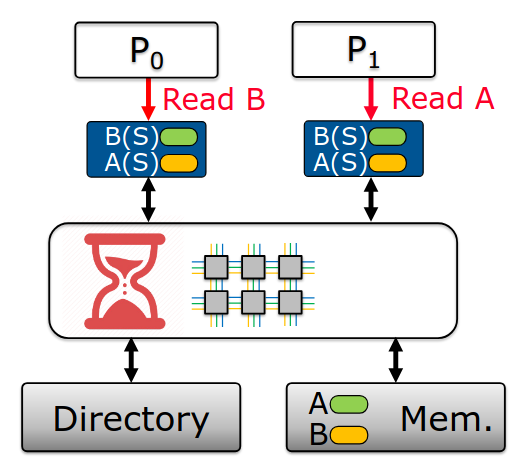
\includegraphics[width=6cm]{images/32.png}
    \end{image}
    
    To avoid this we must define a rigorous memory model to tell each layer what can and can't happen. We'll see different model.
    \subsection{Sequential consistency}
    \begin{tcolorbox}[vert]
        The goal of \important{sequential consistency} is that the multiprocessor should behave like a multi tasked single processor. The result of any execution is the same as if the operations of all processors (cores) were executed in some sequential order, and the operations of each
individual processor (core) appear in this sequence in the order specified by its
program.
    \end{tcolorbox}
    The memory appears like it has a switch in front and like if each processor's memory accesses is executed atomically and in program order.
    \begin{remark}{Remark}
        When we say that it appears atomic, it means that a write transitions directly from “not visible” to “fully visible,” with no observable intermediate state. Then, it ensures that a write is either visible, either invisible, not half-half.
    \end{remark}
    \begin{tcolorbox}[violet]
        To implement sequential consistency we have to ensure two things 
        \begin{enumerate}[left=10pt]
            \item Memory accesses happen in order.
            \item Memory operations appear atomic.
        \end{enumerate}
    \end{tcolorbox}
    To implement, we have to recall that the processor initially act like this
    \begin{center}
        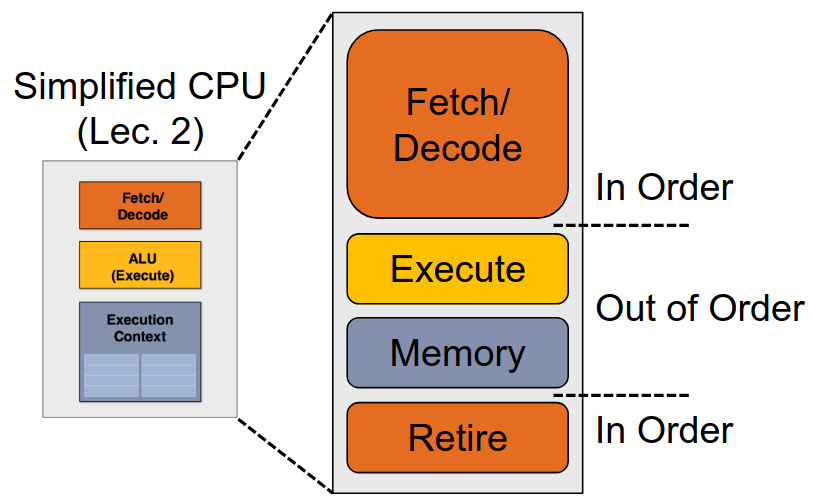
\includegraphics[width=8cm]{images/33.png}
    \end{center}
    \begin{tcolorbox}[vert]
        For the sequential consistency, we need to order memory instructions, using a \important{load-store queue (LSQ)} that will do the following things:
        \begin{itemize} 
            \item Track the FIFO (firs in first out) program order of loads and stores, 
            \item Resolve addresses when they are ready, 
            \item On a load, check for the \textbf{youngest} store to this address.
        \end{itemize}
    \end{tcolorbox}
    \textbf{Load store queue functionality:}

    The LSQ resolves which load/store addresses overlap and hold store operations until they retire. It cannot write ``speculative'' values to caches, a speculative value is a out of order value. It means that the LSQ cannot exit an entry that is still in the ROB.
    \begin{center}
        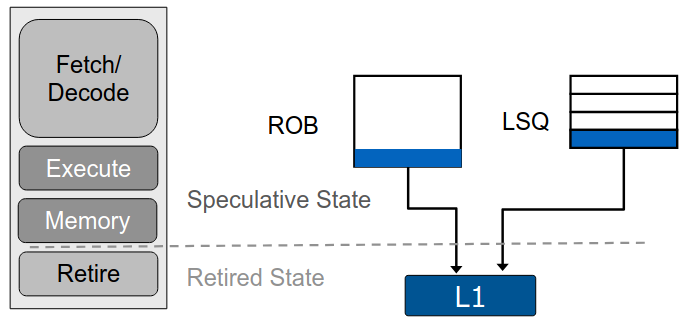
\includegraphics[width=8cm]{images/35.png}
    \end{center}
    
    

    At address resolution of each load, we have to check if there is an older write in the LSQ at the same address. To do this, we use a matrix of comparators, that checks every entry against all older ones. In the example of loads after store, loads sets bits for all older stores they depend on, then the store resets its column when updating the cache (commit).
    \begin{image}{In this picture, each store have its column, when the load address resolution happens, a 1 is set on the column of the store if this is the same address. Then, when the store quit the LSQ, its column is reset to 0.}
        \begin{center}
        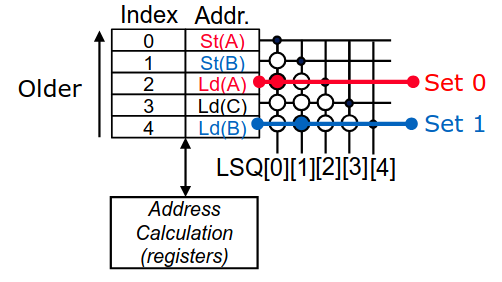
\includegraphics[width=7cm]{images/34.png}
        \end{center}
    \end{image}

        The problem now is that we have to wait for store to complete! If this is a miss in L1/L2/LLC, it can takes 100+ cycles! The goal is that the processor continue while store pending.
        
    \begin{tcolorbox}[vert]
        The solution is to add a \important{store buffer (SB)}. It sits between core and L1 cache and holds committed stores.
    \end{tcolorbox}
    \begin{center}
        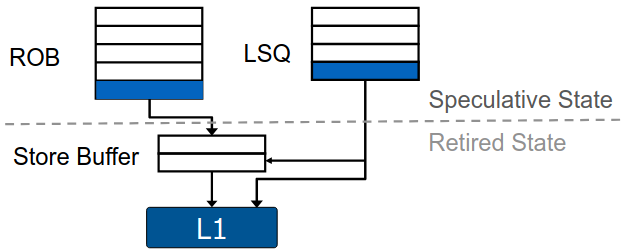
\includegraphics[width=9cm]{images/36.png}
    \end{center}
    \begin{tcolorbox}[gris]
        In the LSQ, we have the address of stalled operations, why not using them?

        We can't because it violates order or atomicity, but, in fact, we can use them by peeking. The idea is to peek at L1, to see if address is already there, if not, we fetch the block from lower level into L1. If the value is there, we \textbf{don't} load the value into the core. Fetching blocks into L1 from lower level or other L1's doesn't impact order or atomicity, there is no values moved between the core and L1. We then can fetch as many blocks in parallel into L1 as needed.
    \end{tcolorbox}

\subsection{Processor consistency}
    \begin{tcolorbox}[vert]
    In processor consistency, reads in the LSQ can bypass writes in the SB.
    \end{tcolorbox}
    If we have instructions in store buffer, then the differences between sequential consistency with peek and processor consistency will be
    \begin{center}
        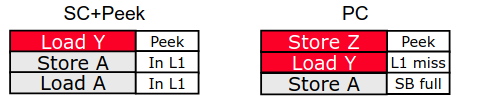
\includegraphics[width=9cm]{images/37.png}
    \end{center}
    In sequential consistency with peeking, load A hits L1, but still had to wait, in processor consistency, load A can bypass stores in the store buffer.

\subsection{Weak consistency}
    \begin{tcolorbox}[vert]
        In \important{weak consistency} there is two sorts of memory operations, data operations or synchronization operations. Only synchronized one have any ordering, data operations have no order enforced among themselves.
    \end{tcolorbox}
    \begin{image}{ Synchronization instructions are called \lstinline!Fences!, it enforces program order for operations before/after.}
    \begin{center}
        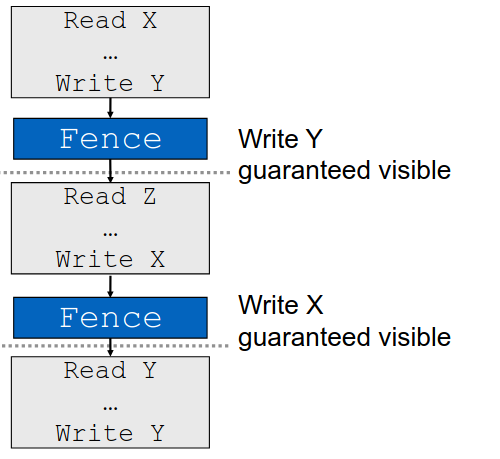
\includegraphics[width=6cm]{images/38.png}
    \end{center}
    \end{image}
   
\subsection{Language level consistency}
    \begin{tcolorbox}[vert]
        A \important{data race} is when two conflicting operations from different threads occur simultaneously. Operations conflict if they access the same location, and at least one is a write and these simultaneous operations are defined back-to-back accesses in any sequentially consistency.
    \end{tcolorbox}
    If we check data races in our \hyperlink{consistency}{\textbf{\textit{first example}}} we can see that there is sequential consistency executions where read/write to A or B are back to back:
    \begin{itemize}[left=10pt, label=\textbullet]
        \item $A=1$
        \item $r_1=B$
        \item $B=1$
        \item $r_2 = A$
    \end{itemize}
    \begin{tcolorbox}[rouge]
        To make a data race free (DRF) code, we can do multiple things. Either we add add fences, by writing these lines: \lstinline! _sync_synchronize();!

        The new way is to declaring \lstinline!A, B! as special variables (e.g. \lstinline!atomic int!).
    \end{tcolorbox}

    \textbf{DRF implies sequential consistency:}

    Before we needed to adjust our programs depending on consistency model in the ISA. But with DRF even on hardware that uses PC or WC, our program sees it as SC, the programmer simply needs to obey the rules.

    \subsubsection{Java Memory Model}

    \begin{tcolorbox}[vert]
        Memory order in Java is defined by \important{``happens-before''} relationship, these defined which re-ordering are possible in both the compiler and the JVM. Without the happens-before guarantee, the compiler/JVM can reorder instructions. From now, we'll write happens-before as an arrow: \textrightarrow. 
    \end{tcolorbox}

    \begin{tcolorbox}[gris]
        There is five situations where \textrightarrow \space is guarantee by Java:
        \begin{itemize}[left=10pt, label=\textbullet]
            \item Actions in the same thread \textrightarrow \space each other in program order. 
            \item Unlock a monitor \textrightarrow \space all locking operations. It means that a thread cannot lock a value if this value is already locked by another thread, it must wait until the other thread unlocks it. 
            \item Writing to a volatile \textrightarrow \space all subsequent reads of that field. 
            \item All actions in a thread \textrightarrow \space a \lstinline!join()! on that thread.
            \item If $A_x$ \textrightarrow \space $A_y$, and $A_y$ \textrightarrow \space $A_z$, then $A_x$ \textrightarrow \space $A_z$.
        \end{itemize}
    \end{tcolorbox}

    If we can find two actions $A_x$ such that $A_x$ doesn't \textrightarrow \space $A_y$, and $A_y$ doesn't \textrightarrow \space $A_x$, we have found a data race.
    \begin{center}
    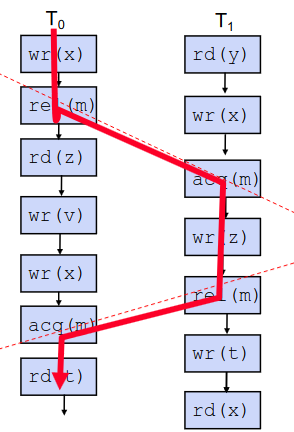
\includegraphics[width=4cm]{images/39.png}
    \end{center}
    \begin{image}{But sometimes, some actions may or may not happens before another. Then, \lstinline!wr(t)! is not guaranteed to happens before \lstinline!rd(t)!, so there is data race.}
        \begin{center}
        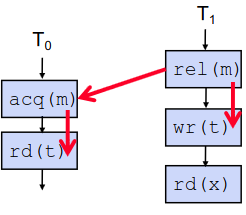
\includegraphics[width=3cm]{images/40.png}
        \end{center}
    \end{image}
    To eliminate data race we can just add \lstinline!synchronized { }! blocks or \lstinline!@volatile! variables.

    \textbf{Synchronized blocks versus volatile:}
    \begin{tcolorbox}[gris]
    Synchronized blocks can only works with objects, the thread can wait while others are in synchronized blocks and they can wrap whole functions or critical sections.
    \begin{image}{On this code, another thread will either see both a and x to be updated neither a nor x to be updated}
        \begin{codeCenter}
        \begin{Ccode}
synchronized {
    a = b + c;
    x = foo ();
}
        \end{Ccode}
        \end{codeCenter}
    \end{image}
    \end{tcolorbox}
    \begin{tcolorbox}[gris]
        Volatile can be used with primitives (e.g. \lstinline!int!), there is no synchronization/direct access and it prevents specific memory re-ordering.
        \begin{image}{If another thread sees x to be updated it must also see a to be updated. But reverse is not necessarily true.}
            \begin{codeCenter}
            \begin{Ccode}
@volatile int a, x;
a = b + c;
x = foo();
// can't reorder before 
// wr(a)
            \end{Ccode}
            \end{codeCenter}
        \end{image}
    \end{tcolorbox}
\subsubsection{C++ 11 Memory Model}
    All thread can read/write to any location in the program scope through references and pointers, it's way more permissive than Java. Data races are similarly defined: we recall that a data race occurs when two conflicting memory operations that do not operate on ``special'' variables happens.  

    The equivalent of a volatile variable is a \lstinline!std::atomic<T>! to designate a special variable of type T. The equivalent of synchronized blocks is defined as \lstinline!std::mutex(...)!.
\subsubsection{OpenMP Memory Model}
    Since OMP is yet another threading library its memory model differs from C++ 11. There is no concept of a synchronization variable like \lstinline!@volatile! or \lstinline!std::atomic<T>!. Locks must be accompanied by a flush (ex. to come).

    Officially, OMP implements weak consistency except for flush operations.

    \begin{tcolorbox}[rouge]
    \begin{image}{When we writing code, we need to consider data races only on shared variables.}
        \begin{codeCenter}
        \begin{Ccode}
#pragma omp parallel
private (x) shared (y)
{
    x = ...
    *y++; //data race
}
        \end{Ccode}
        \end{codeCenter}
    \end{image}
    \end{tcolorbox}
    \begin{tcolorbox}[vert]
        A \important{flush} is a memory fence.
    \end{tcolorbox}
    \begin{image}{In order to communicate between threads, they do the following: first thread writes the shared variable, then flushes the variable and the second thread flushes and then reads.}
        \begin{codeCenter}
        \begin{Ccode}
int y;
#pragma omp parallel shared(y)
{
    if( thr_id == 0 ) {
    y = ...;
    #pragma omp flush(y)
}
    #pragma omp flush(y)
    ... = y;
}
        \end{Ccode}
        \end{codeCenter}
    \end{image}
 
